\section{Experiments and Results}
\label{sec:exp}
% [12 pts] Task 1: trajectories, CD. Task 2: loss, FID vs CFG, steps.
% Task 3: FID comparison, speed-up, straightness. Task 4: full pipeline.

\begin{figure*}[t]
  \centering
  \begin{subfigure}{0.245\linewidth}
    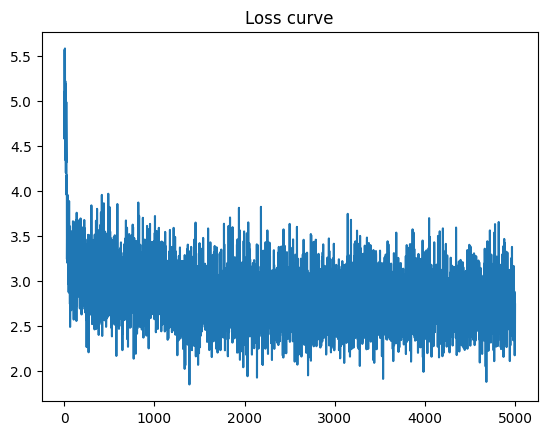
\includegraphics[width=\linewidth]{Figure/task1_loss.png}
    \caption{Task 1 (2D FM)}
  \end{subfigure}\hfill
  \begin{subfigure}{0.245\linewidth}
    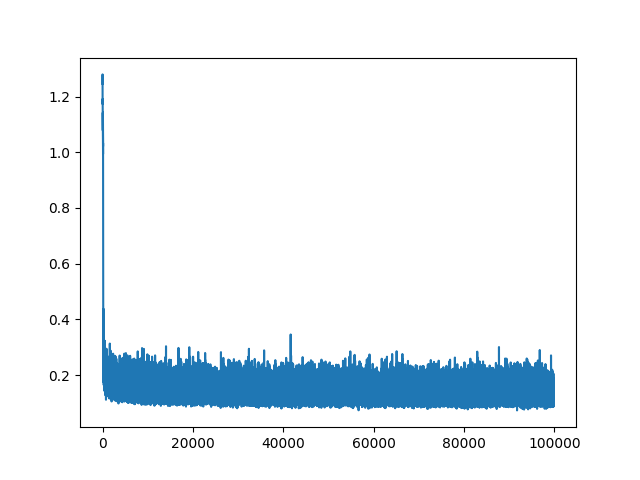
\includegraphics[width=\linewidth]{Figure/task2_loss.png}
    \caption{Task 2 (image FM)}
  \end{subfigure}\hfill
  \begin{subfigure}{0.245\linewidth}
    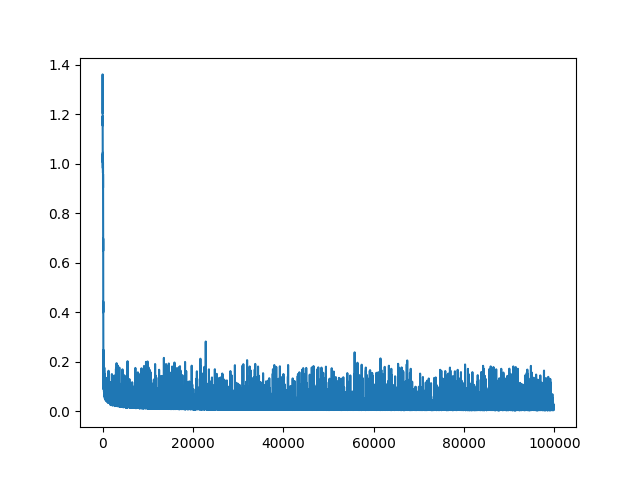
\includegraphics[width=\linewidth]{Figure/task3_loss.png}
    \caption{Task 3 (1-RF)}
  \end{subfigure}\hfill
  \begin{subfigure}{0.245\linewidth}
    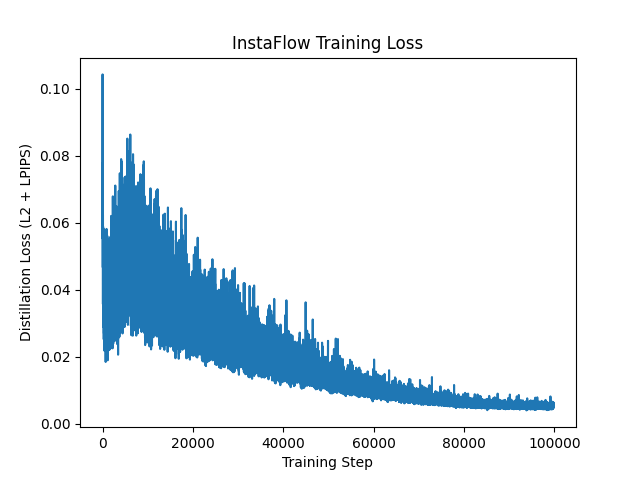
\includegraphics[width=\linewidth]{Figure/task4_loss.png}
    \caption{Task 4 (InstaFlow)}
  \end{subfigure}
  \caption{\textbf{Training loss curves} (x-axis: training step). The FM losses plateau at a non-zero value because a point $x_t$ is reachable from many random $(x_0,x_1)$ pairs; with the reflow pairs of Task 3 this ambiguity mostly disappears and the loss is about $10\times$ lower. The bump in Task 4 comes from the 5k-step learning-rate warm-up.}
  \label{fig:loss}
\end{figure*}

\subsection{Task 1: 2D Flow Matching}
\begin{figure*}[t]
  \centering
  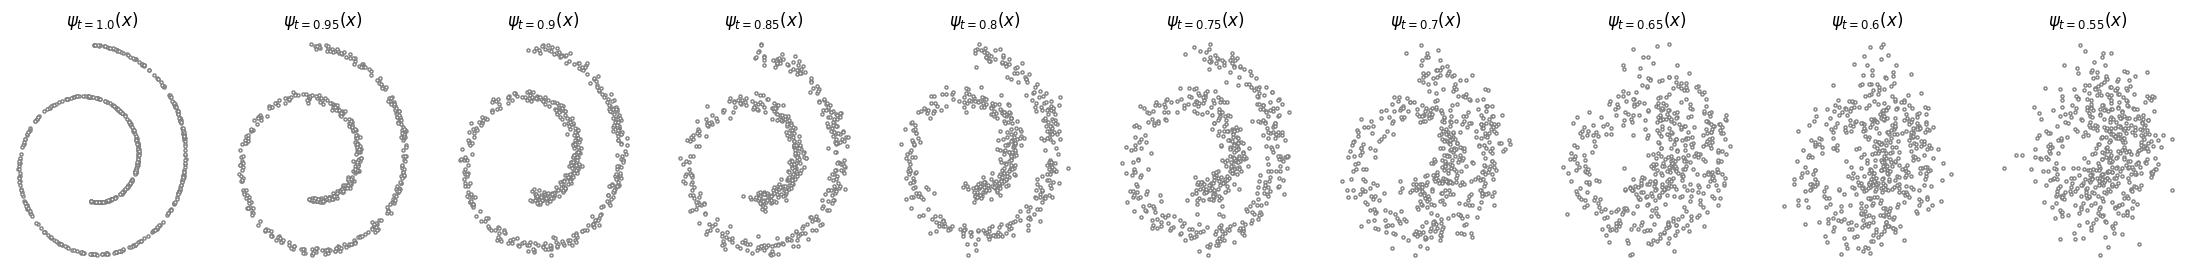
\includegraphics[width=\linewidth]{Figure/task1_psi.png}
  \caption{\textbf{Task 1: conditional path} $\psi_t(x_0\mid x_1)$ applied to Swiss-roll samples, from $t=1$ (data) to $t=0.55$. Points move linearly toward the Gaussian prior.}
  \label{fig:psi}
\end{figure*}

\begin{figure*}[t]
  \centering
  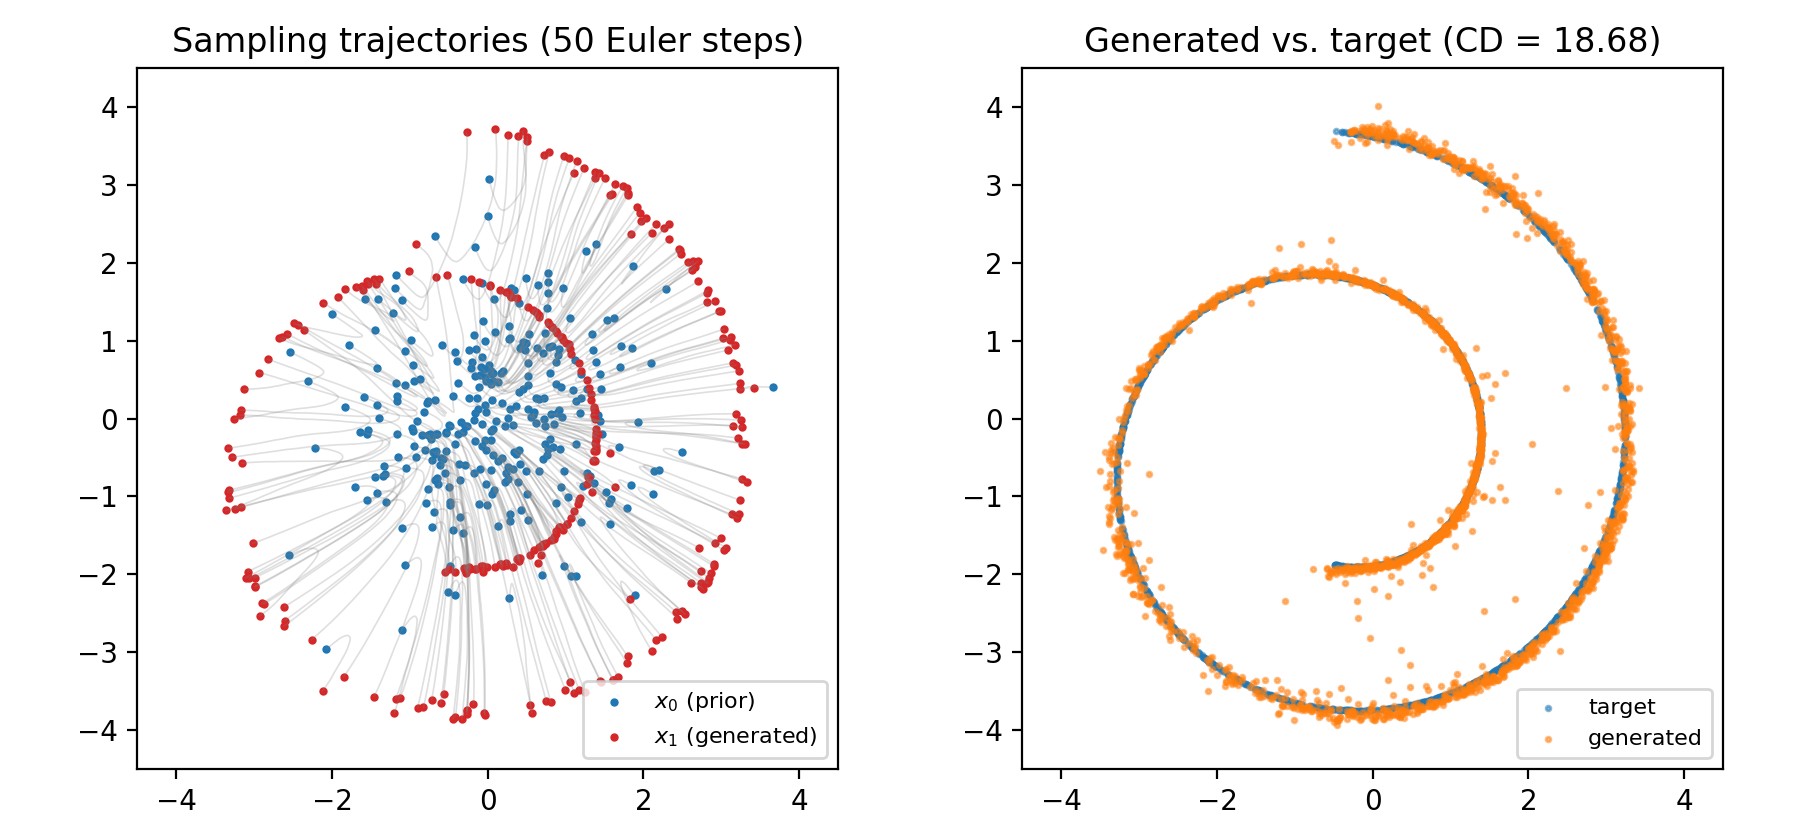
\includegraphics[width=0.72\linewidth]{Figure/task1_traj.png}
  \caption{\textbf{Task 1: learned trajectories.} Left: 300 sampling trajectories from the prior (blue) to the generated points (red). Right: 2,048 generated points against the target. This figure is from a re-run with the same configuration (CD 18.68); the graded notebook run reached CD 13.49.}
  \label{fig:task1}
\end{figure*}

The notebook trains for 5k iterations and evaluates the Chamfer distance (CD) between 2,048 generated and 2,048 target points with 50 Euler steps, giving \textbf{CD = 13.49} ($<40$, full score).
\Cref{fig:psi} visualizes the conditional path and \cref{fig:task1} the learned flow.
The trajectories are nearly straight near the prior but bend near the end, where points must choose an arm of the spiral; this curvature is what Rectified Flow later reduces.
Only a few points fall between the arms, which is the main source of the remaining CD.

\subsection{Task 2: Image Flow Matching with CFG}
\begin{table}[t]
  \centering
  \footnotesize
  \caption{\textbf{Task 2: FID} ($\downarrow$) of the base FM model, 500 samples. NFE: network evaluations per sample (CFG doubles it).}
  \label{tab:task2}
  % values: results/cfg_fm-11-01-023216/eval/fid_results.txt
  \begin{tabular}{@{}lccc@{}}
    \toprule
    Setting & Steps & NFE & FID \\
    \midrule
    CFG 1.0 & 20 & 20  & 12.18 \\
    CFG 3.0 & 20 & 40  & 12.13 \\
    \textbf{CFG 7.5} & \textbf{20} & \textbf{40} & \textbf{7.39} \\
    \midrule
    CFG 7.5 & 10 & 20  & 8.14 \\
    CFG 7.5 & 50 & 100 & 5.47 \\
    \bottomrule
  \end{tabular}
\end{table}


\begin{figure*}[t]
  \centering
  \begin{subfigure}{0.49\linewidth}
    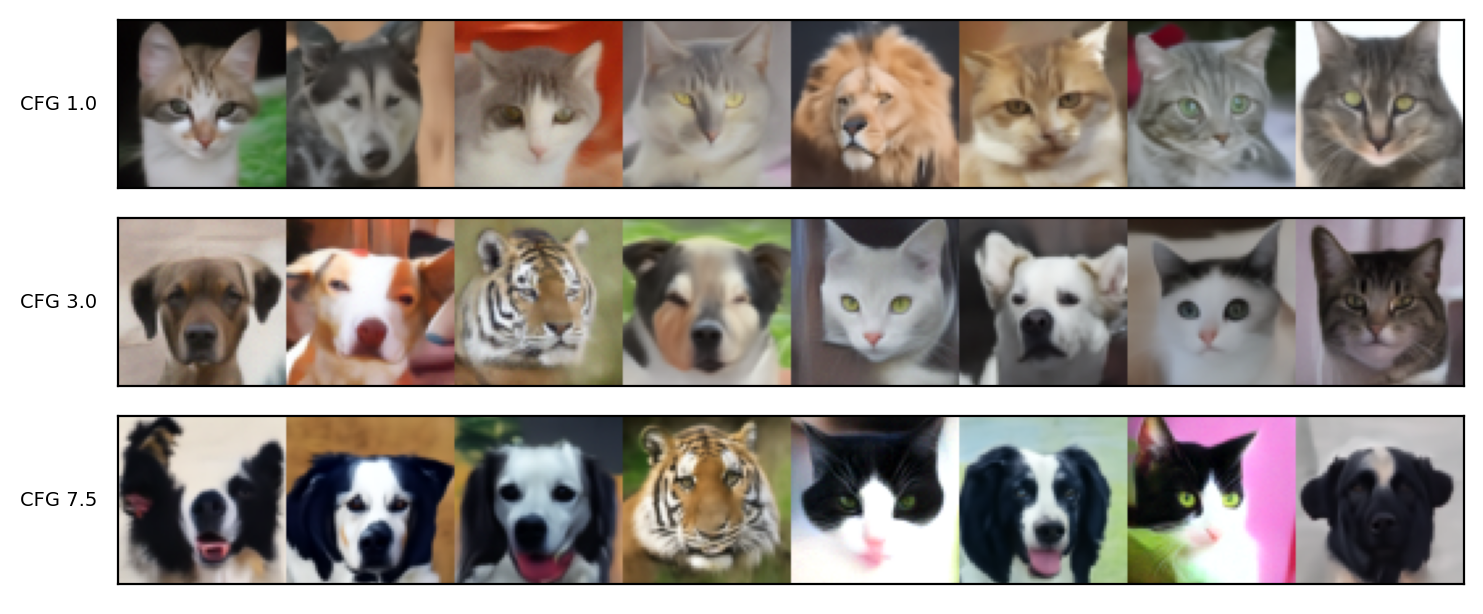
\includegraphics[width=\linewidth]{Figure/task2_cfg.png}
    \caption{CFG scale (20 steps)}
  \end{subfigure}\hfill
  \begin{subfigure}{0.49\linewidth}
    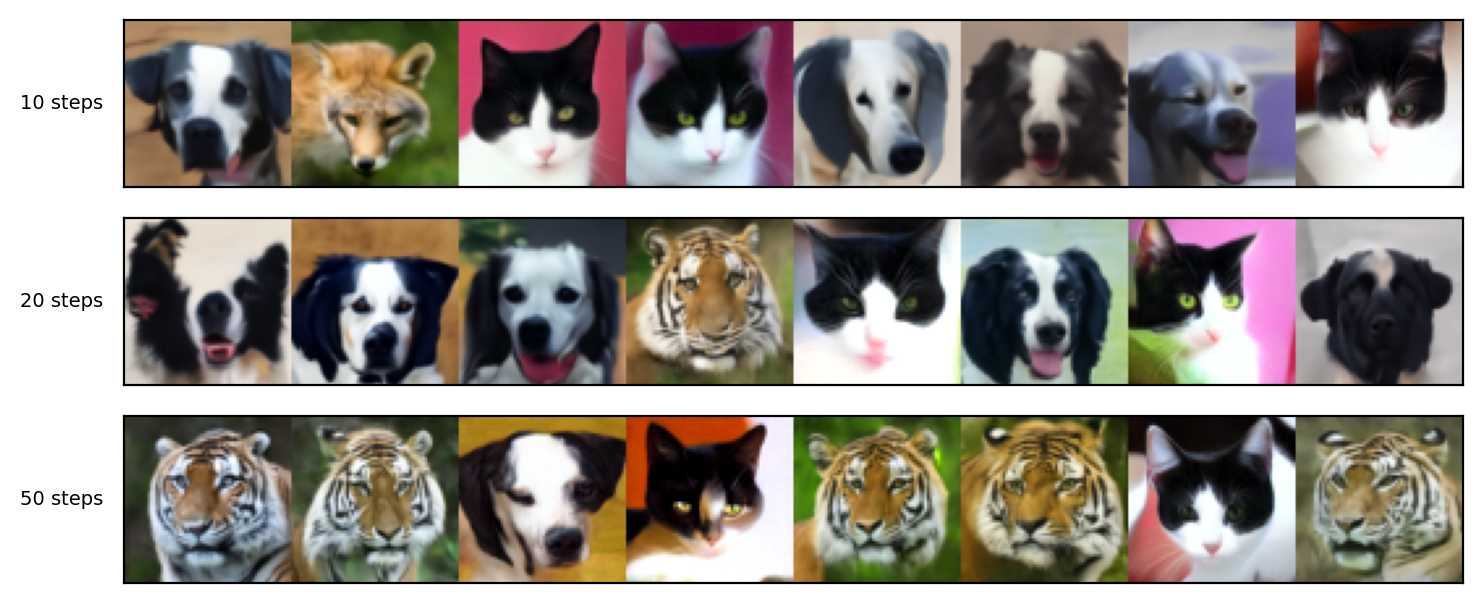
\includegraphics[width=\linewidth]{Figure/task2_steps.png}
    \caption{Number of steps (CFG 7.5)}
  \end{subfigure}
  \caption{\textbf{Task 2 samples} of the base FM model. Samples in different rows come from different noise.}
  \label{fig:task2}
\end{figure*}

\Cref{tab:task2} reports FID for different CFG scales and step counts, and \cref{fig:task2} shows samples.
\textbf{CFG 7.5 with 20 steps reaches FID 7.39} ($<30$, full score).
\begin{itemize}
  \item \textbf{CFG scale.} Larger guidance lowers FID (12.18 $\rightarrow$ 7.39).
  Visually, CFG 1.0 produces diverse but blurrier animals, while CFG 7.5 produces sharp, high-contrast faces that are less diverse (many black-and-white cats and dogs, saturated backgrounds).
  \item \textbf{Steps.} More steps help (10: 8.14, 20: 7.39, 50: 5.47), and the cost grows linearly with the number of network evaluations.
  The small gap between 10 and 20 steps already suggests that the learned trajectories are fairly straight.
\end{itemize}

\subsection{Task 3: Rectified Flow}
\begin{table}[t]
  \centering
  \footnotesize
  \setlength{\tabcolsep}{4pt}
  \caption{\textbf{Task 3: Base FM vs.\ 1-Rectified Flow} at CFG 7.5. FID ($\downarrow$) on 500 samples; time is wall-clock for the 500 samples. Both models share the architecture, so the time per step is identical.}
  \label{tab:task3}
  % values: results/rectified_fm_1-11-01-151854/eval/{fid_results.txt,evaluation_results.json}
  \begin{tabular}{@{}ccccc@{}}
    \toprule
    & \multicolumn{2}{c}{FID} & \multicolumn{2}{c}{Time (s)} \\
    \cmidrule(lr){2-3}\cmidrule(l){4-5}
    Steps & Base FM & 1-RF & Base FM & 1-RF \\
    \midrule
    5  & 8.72 & \textbf{5.52} & 14.4 & 14.2 \\
    10 & 9.16 & \textbf{3.35} & 28.5 & 28.5 \\
    20 & 5.84 & \textbf{3.29} & 56.9 & 57.0 \\
    \bottomrule
  \end{tabular}
\end{table}

\begin{table}[t]
  \centering
  \footnotesize
  \caption{\textbf{Trajectory straightness} $S$ ($\downarrow$, \cref{eq:straight}) over 256 trajectories of 20 Euler steps, using the same noise and labels for both models.}
  \label{tab:straight}
  % values: report/Figure/analysis_results.json
  \begin{tabular}{@{}lcc@{}}
    \toprule
    Sampling guidance & Base FM & 1-RF \\
    \midrule
    CFG 1.0 (learned field) & 0.0222 & \textbf{0.0016} \\
    CFG 7.5                 & \textbf{0.0419} & 0.5946 \\
    \bottomrule
  \end{tabular}
\end{table}


\begin{figure*}[t]
  \centering
  \begin{subfigure}[b]{0.52\linewidth}
    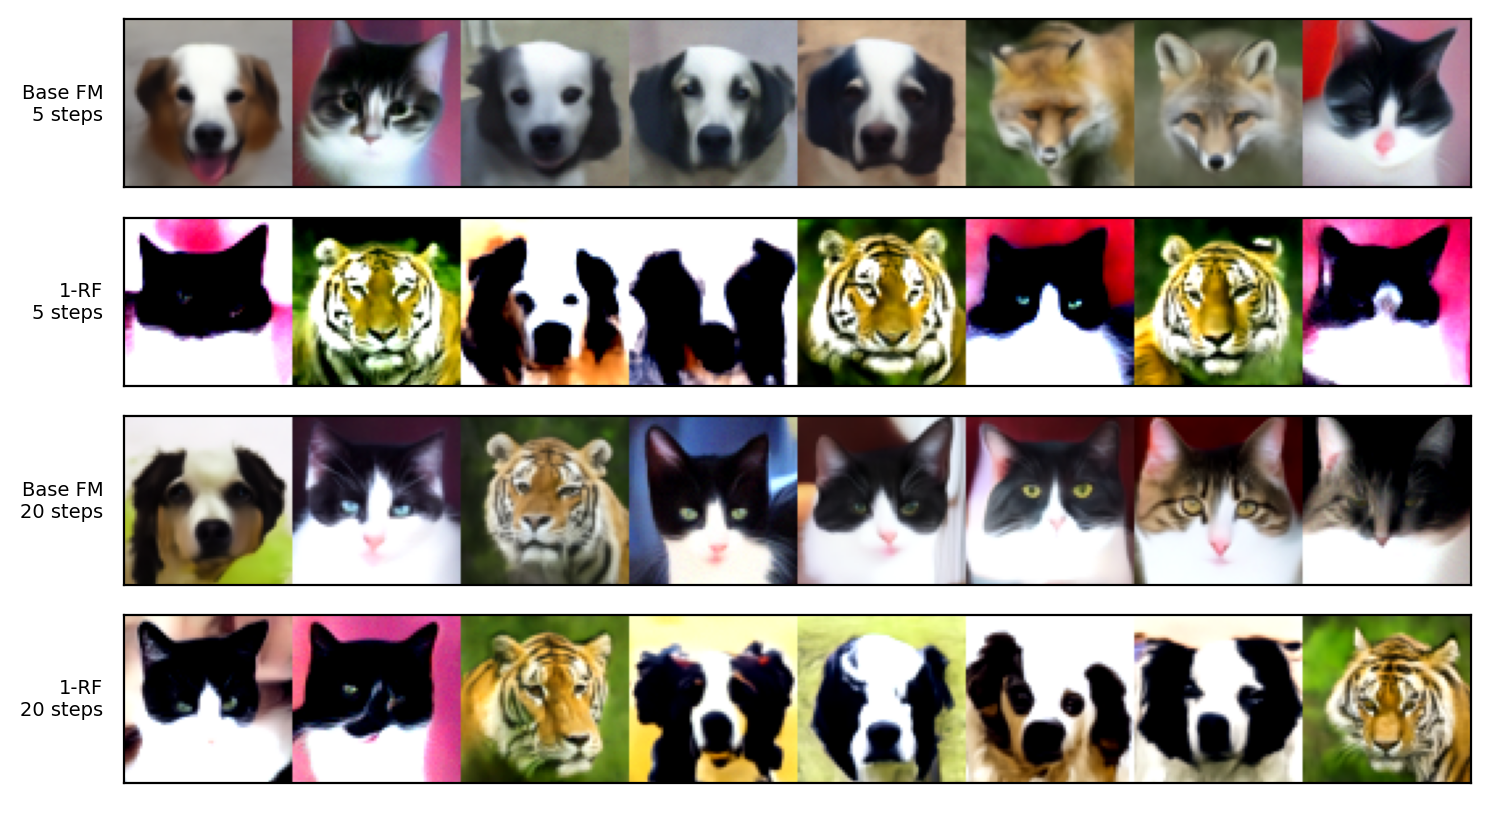
\includegraphics[width=\linewidth]{Figure/task3_samples.png}
    \caption{Samples (CFG 7.5) with 5 and 20 steps.}
    \label{fig:task3}
  \end{subfigure}\hfill
  \begin{subfigure}[b]{0.44\linewidth}
    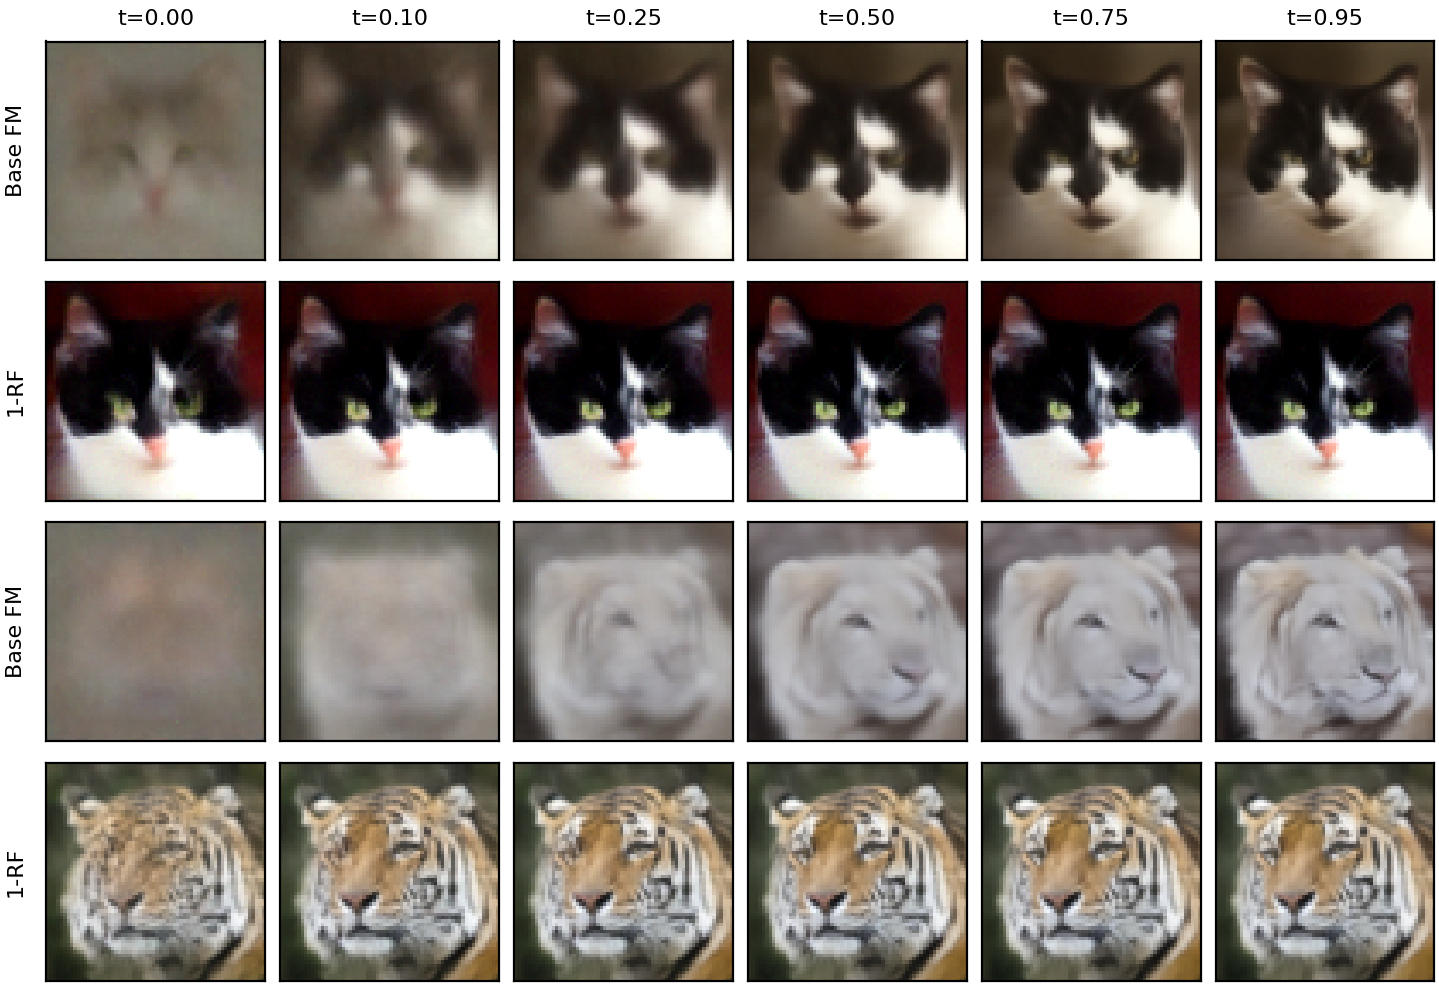
\includegraphics[width=\linewidth]{Figure/task3_x1hat.png}
    \caption{Predicted endpoint along a trajectory (CFG 1.0).}
    \label{fig:x1hat}
  \end{subfigure}
  \caption{\textbf{Task 3: base FM vs.\ 1-RF.} (b) shows the predicted endpoint $\hat x_1=x_t+(1-t)\,v_t$ for the same noise: base FM starts from a blurry average and commits to details only gradually, while 1-RF already knows the final image at $t=0$, \ie its trajectory is almost a straight line.}
\end{figure*}

\paragraph{FID and speed.}
\Cref{tab:task3} compares the two models at the same step counts.
\textbf{1-RF reaches FID 5.52 with only 5 steps} ($<30$, full score), about the same as base FM with 20 steps (5.84).
Since both models share the architecture, the time per step is identical; the speed-up comes from needing fewer steps.
For similar quality (\cref{fig:fid_time}), 1-RF with 5 steps takes 14.2\,s versus 56.9\,s for base FM with 20 steps, a \textbf{$\sim$4$\times$ speed-up}.
1-RF also barely improves from 10 to 20 steps (3.35 $\rightarrow$ 3.29), so additional steps have little left to correct.
Note that the reflow targets were generated with CFG 7.5 and CFG 7.5 is applied again at evaluation, and 500-sample FIDs are noisy (\eg base FM at 5 vs.\ 10 steps), so small FID differences should not be over-interpreted.

\begin{figure}[t]
  \centering
  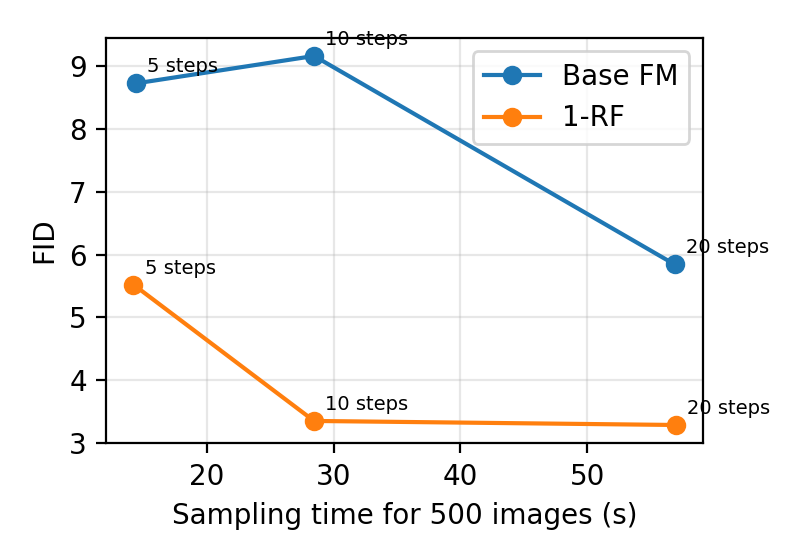
\includegraphics[width=0.9\linewidth]{Figure/task3_fid_time.png}
  \caption{\textbf{Task 3: quality vs.\ sampling time} (CFG 7.5, 500 images). 1-RF reaches with 5 steps the FID that base FM needs 20 steps for.}
  \label{fig:fid_time}
\end{figure}

\paragraph{Trajectory straightness.}
Following~\cite{liu2023rectified}, I measure how far the velocity deviates from the overall displacement along a trajectory,
\begin{equation}
  S = \mathbb E_{t}\big\|(x_1-x_0) - v_t\big\|^2,
  \label{eq:straight}
\end{equation}
averaged per pixel ($S=0$ for a straight line).
Without guidance, 1-RF is about \textbf{14$\times$ straighter} than base FM (\cref{tab:straight}), which \cref{fig:x1hat} shows visually.
With CFG 7.5, however, 1-RF has a large $S$: almost all of the deviation is in the \emph{first} step, where the conditional and unconditional velocities differ strongly and CFG amplifies the gap by $7.5\times$; the remaining steps are straight.
This matters for Task 4 (\cref{sec:discussion}).

\begin{table}[t]
  \centering
  \footnotesize
  \setlength{\tabcolsep}{4pt}
  \caption{\textbf{Task 3: FID with and without guidance} (500 samples). $^\dagger$Most samples are saturated or blurry (\cref{fig:few_steps}); FID fails to reflect this, so these entries are not meaningful.}
  \label{tab:task3_cfg}
  % values: results/rectified_fm_1-11-01-151854/{eval,eval_cfg1.0,eval_cfg7.5_few}/fid_results.txt
  \begin{tabular}{@{}ccccc@{}}
    \toprule
    & \multicolumn{2}{c}{CFG 1.0} & \multicolumn{2}{c}{CFG 7.5} \\
    \cmidrule(lr){2-3}\cmidrule(l){4-5}
    Steps & Base FM & 1-RF & Base FM & 1-RF \\
    \midrule
    1  & 94.64 & \textbf{17.67} & 46.28 & 8.56$^\dagger$ \\
    2  & 80.88 & \textbf{10.14} & 9.07$^\dagger$ & 10.57$^\dagger$ \\
    5  & 36.56 & \textbf{8.07}  & 8.72 & \textbf{5.52} \\
    10 & 17.06 & \textbf{7.26}  & 9.16 & \textbf{3.35} \\
    20 & 11.05 & \textbf{6.96}  & 5.84 & \textbf{3.29} \\
    \bottomrule
  \end{tabular}
\end{table}


\begin{figure*}[t]
  \centering
  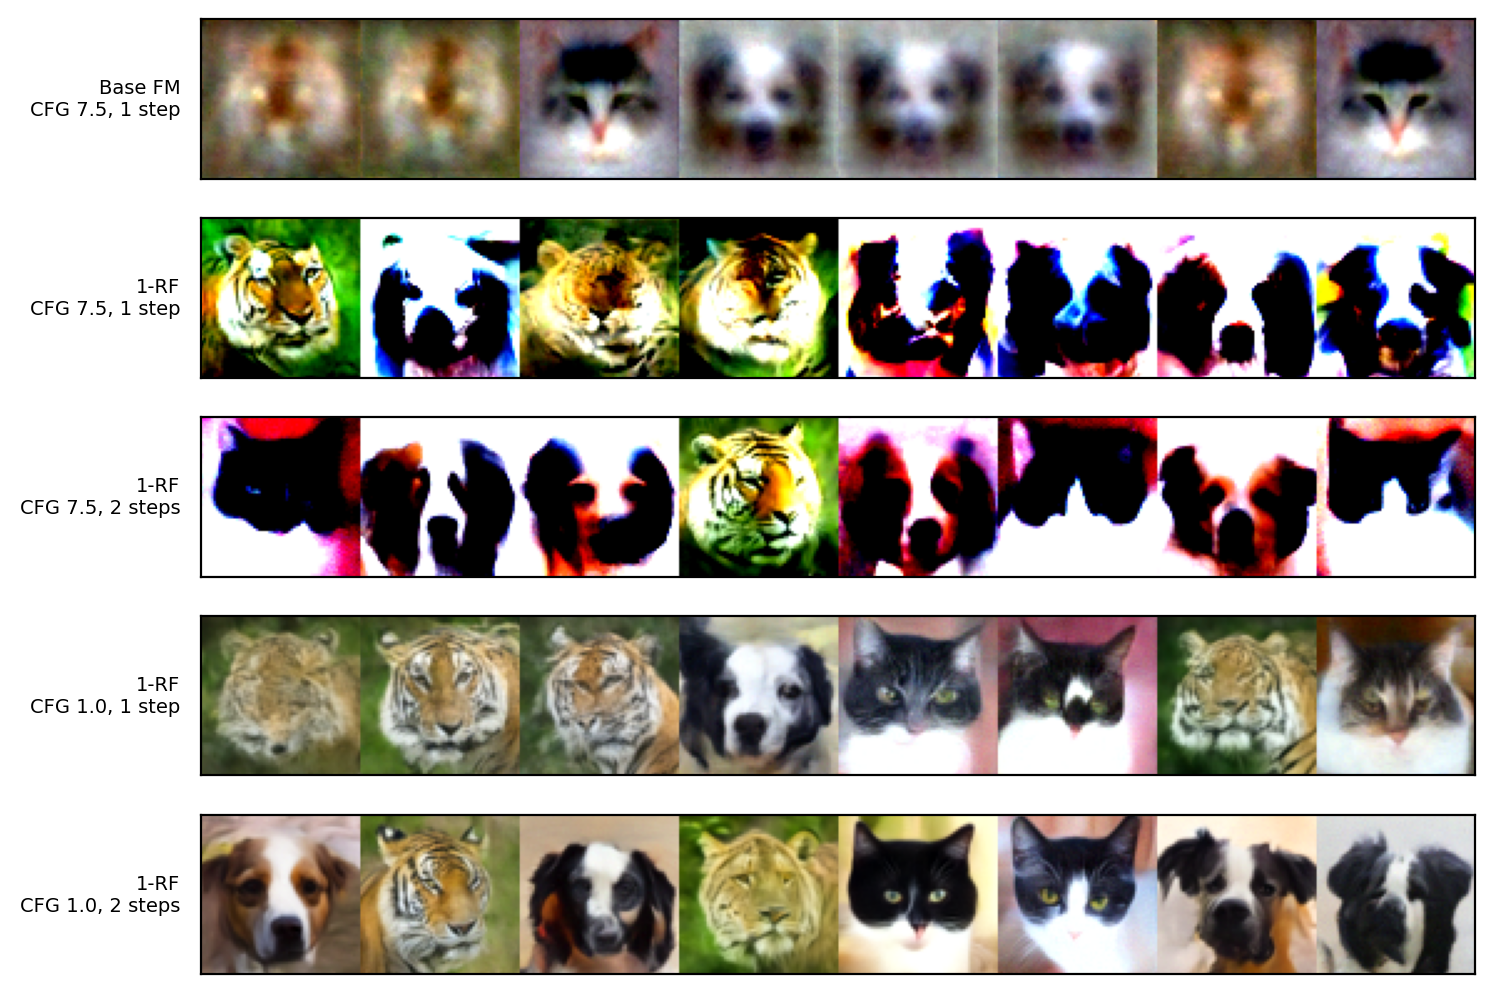
\includegraphics[width=0.75\linewidth]{Figure/task3_few_steps.png}
  \caption{\textbf{Task 3: 1--2 step sampling with and without CFG.} With CFG 7.5, the single large first step of 1-RF overshoots and most images saturate; without guidance 1-RF already produces clean animals in one or two steps. Base FM with one step only produces a blurry average.}
  \label{fig:few_steps}
\end{figure*}

\paragraph{Sampling without guidance.}
Since the reflow targets were generated with CFG 7.5, I also evaluate both models at CFG 1.0 (\cref{tab:task3_cfg}).
Here the gap is much larger: \textbf{1-RF reaches FID 17.67 with one step and 10.14 with two}, while base FM needs 20 steps for 11.05.
At 20 steps, 1-RF without guidance (6.96) matches its teacher (Task 2, CFG 7.5: 7.39), confirming that the guidance is baked into the 1-RF weights; adding CFG 7.5 on top still lowers FID for $\geq$5 steps.
With 1--2 steps, however, CFG 7.5 breaks 1-RF (\cref{fig:few_steps}): the amplified first-step jump pushes pixels out of range.
These broken samples still get a low FID, showing that 500-sample FID is unreliable for such failure modes.

\subsection{Task 4 (Bonus): InstaFlow}
\begin{table}[t]
  \centering
  \footnotesize
  \setlength{\tabcolsep}{2.5pt}
  \caption{\textbf{Task 4: full pipeline.} FID ($\downarrow$) on 500 samples. Timing for 500 samples was measured in one process on the same GPU (batch 128). Speed-up is relative to base FM (50 steps) and to the 1-RF teacher (20 steps).}
  \label{tab:task4}
  % values: results/instaflow-11-01-233319/eval/fid_results.txt, report/Figure/analysis_results.json
  \begin{tabular}{@{}lcccccc@{}}
    \toprule
    Model & Steps & NFE & FID & Img/s & vs.\ FM & vs.\ 1-RF \\
    \midrule
    Base FM (CFG 7.5)  & 50 & 100 & 5.47 & 2.9 & 1$\times$ & -- \\
    1-RF (CFG 1.5)     & 20 & 40  & 5.54 & 7.1 & 2.5$\times$ & 1$\times$ \\
    \textbf{InstaFlow} & \textbf{1} & \textbf{1} & \textbf{7.38} & \textbf{284} & \textbf{99.6$\times$} & \textbf{39.9$\times$} \\
    \bottomrule
  \end{tabular}
\end{table}


\begin{figure*}[t]
  \centering
  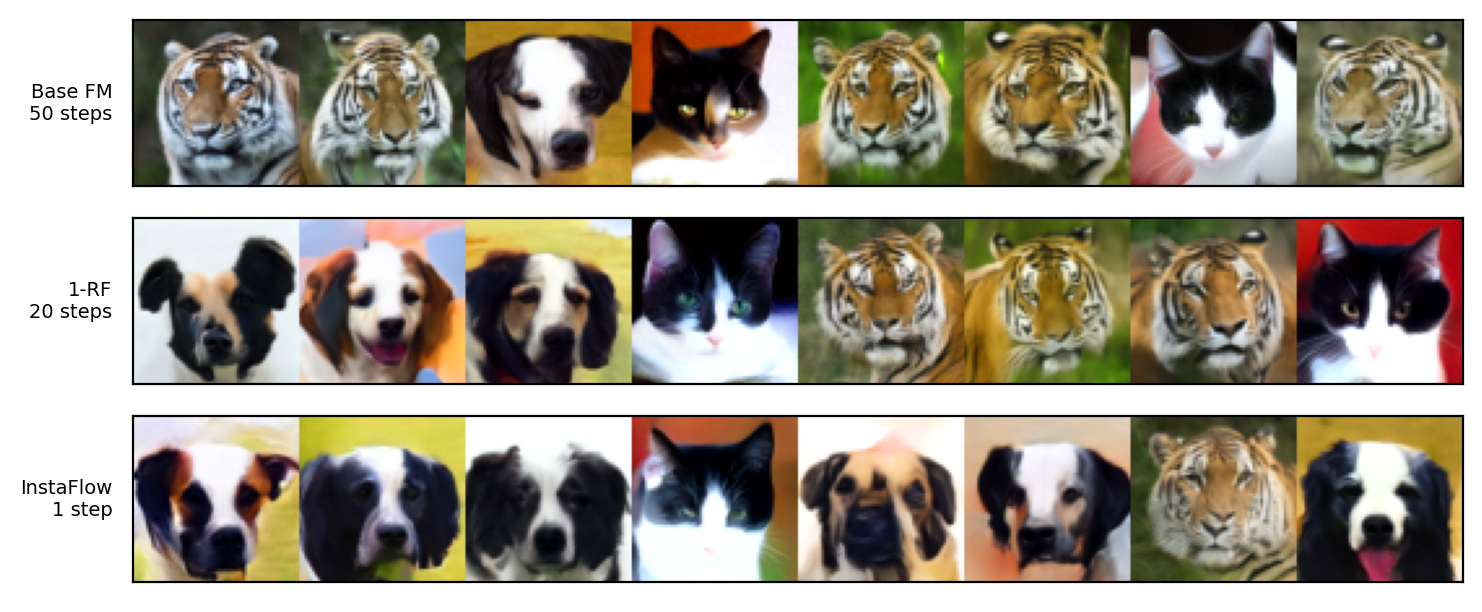
\includegraphics[width=0.75\linewidth]{Figure/task4_samples.png}
  \caption{\textbf{Task 4 samples} from each stage of the pipeline: base FM (100 NFE), 1-RF teacher (40 NFE) and the one-step InstaFlow student (1 NFE).}
  \label{fig:task4}
\end{figure*}

\begin{figure*}[t]
  \centering
  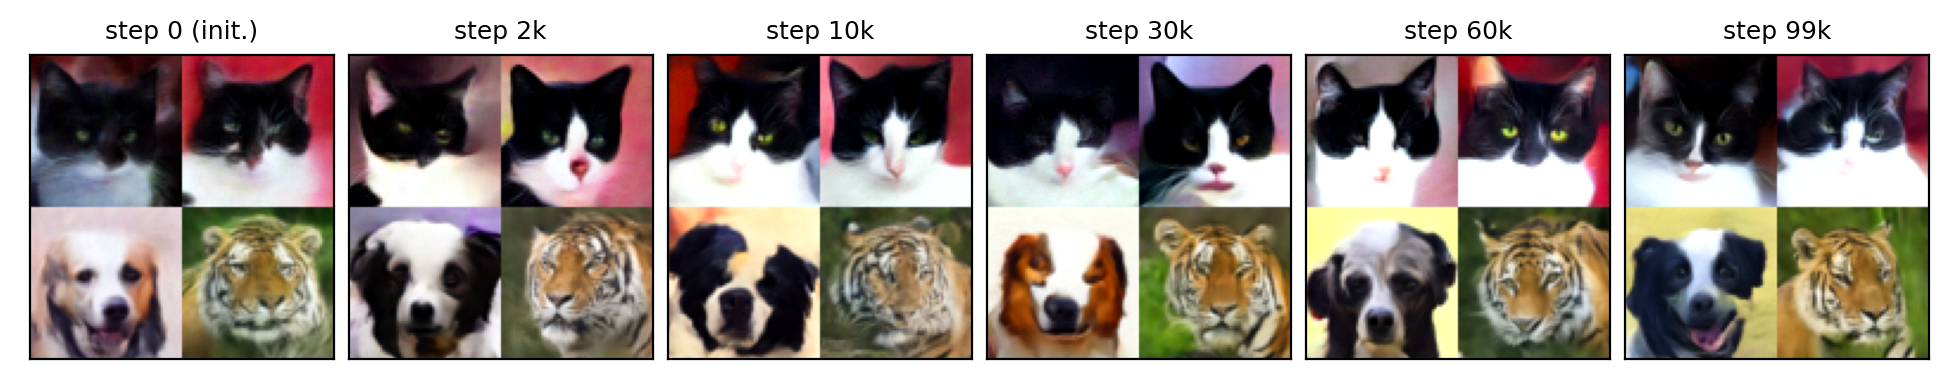
\includegraphics[width=0.9\linewidth]{Figure/task4_progress.png}
  \caption{\textbf{Task 4: one-step samples during distillation} (fixed labels cat, cat, dog, wild). Thanks to the 1-RF initialization, the student generates plausible animals at step 0; distillation mainly sharpens details and removes artifacts.}
  \label{fig:progress}
\end{figure*}

\Cref{tab:task4} summarizes all stages.
\textbf{InstaFlow reaches FID 7.38 with a single step} ($<30$, full bonus), while generating 284 images/s: \textbf{99.6$\times$ faster} than base FM with 50 steps and \textbf{39.9$\times$ faster} than its 1-RF teacher.
The cost is a moderate quality drop (FID 5.47/5.54 $\rightarrow$ 7.38).
\Cref{fig:task4} shows no mode collapse: the one-step samples cover cats, dogs and wild animals with varied colors, but they are slightly blurrier than the multi-step samples.
Because the student is initialized from the 1-RF teacher, it already produces recognizable animals in one step before any distillation update (initial loss 0.08, final 0.005; \cref{fig:progress}), so training only has to refine an already reasonable map.

\begin{table}[t]
  \centering
  \footnotesize
  \setlength{\tabcolsep}{3pt}
  \caption{\textbf{Task 4 ablation.} Each variant changes one setting of the full model and is otherwise identical (same distillation data, 100k steps, seed). Loss is averaged over 500 steps (10 at step 0); it includes the LPIPS term except in the L2-only row, so that row is not comparable. FID ($\downarrow$) on 500 one-step samples.}
  \label{tab:ablation}
  % values: task4_run.log, task4_ablation_{no_lpips,no_init}.log, results/instaflow-*/eval/fid_results.txt
  \begin{tabular}{@{}lcccc@{}}
    \toprule
    & \multicolumn{3}{c}{Training loss at step} & \\
    \cmidrule(lr){2-4}
    Variant & 0 & 20k & 100k & FID \\
    \midrule
    Full (L2 + LPIPS, 1-RF init) & 0.080 & 0.031 & 0.005 & 7.38 \\
    L2 only                      & 0.020 & 0.006 & 0.001 & 6.92 \\
    Random init                  & 2.463 & 0.071 & 0.009 & 7.31 \\
    \bottomrule
  \end{tabular}
\end{table}


\begin{figure*}[t]
  \centering
  \begin{subfigure}[b]{0.52\linewidth}
    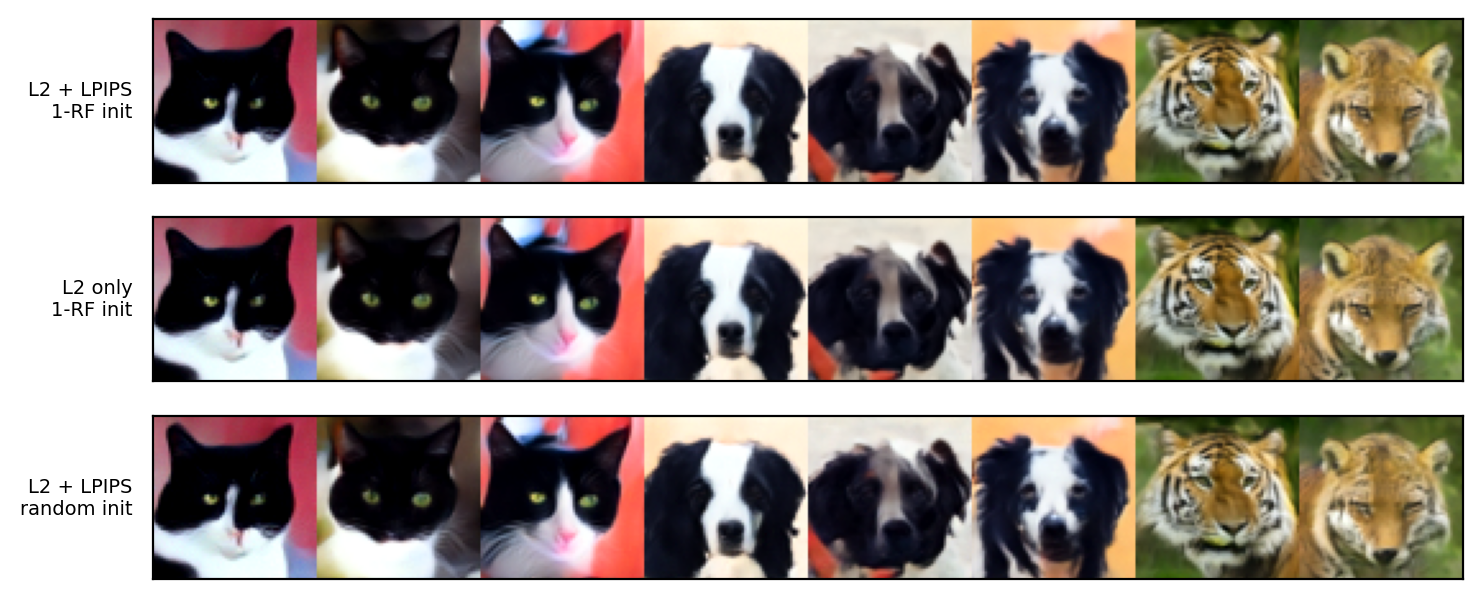
\includegraphics[width=\linewidth]{Figure/task4_ablation_samples.png}
    \caption{Final one-step samples from the same noise and labels.}
    \label{fig:abl_samples}
  \end{subfigure}\hfill
  \begin{subfigure}[b]{0.46\linewidth}
    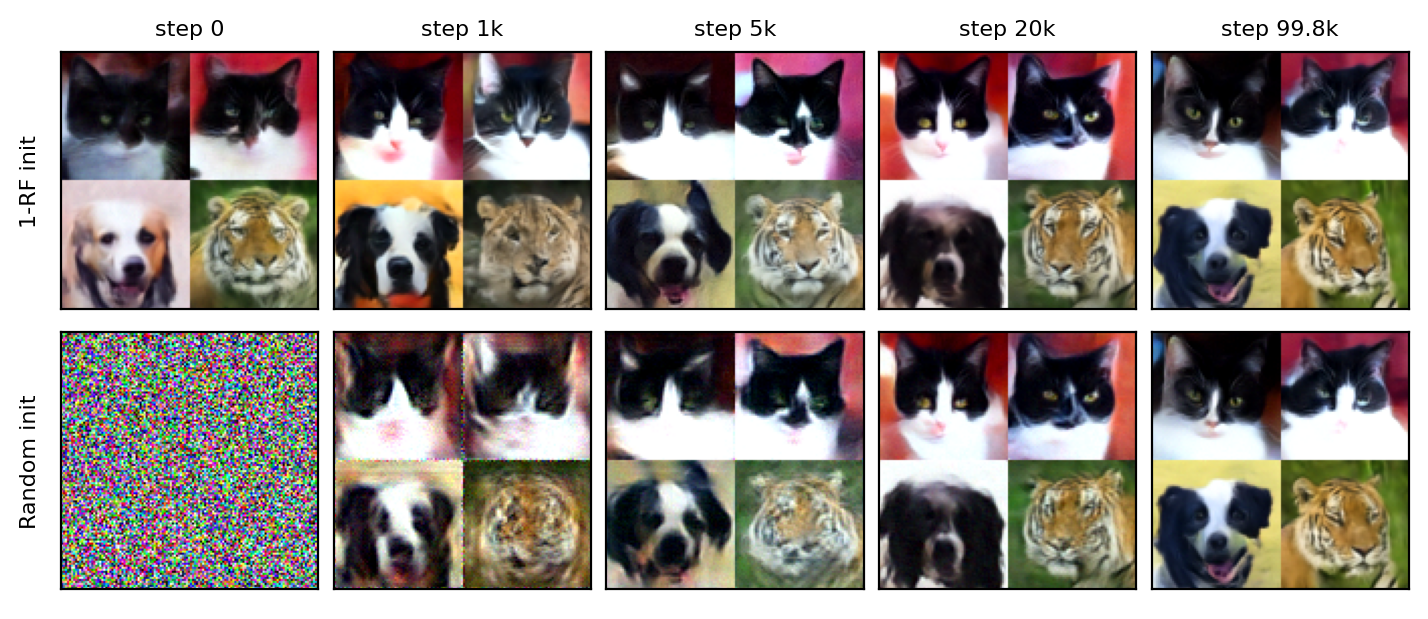
\includegraphics[width=\linewidth]{Figure/task4_ablation_progress.png}
    \caption{Samples during training, with and without 1-RF init.}
    \label{fig:abl_progress}
  \end{subfigure}
  \caption{\textbf{Task 4 ablation.} (a) All three students converge to almost the same one-step map. (b) The randomly initialized student starts from noise and is blurry at 1k steps, but catches up with the 1-RF-initialized one by about 5--20k steps.}
  \label{fig:ablation}
\end{figure*}

\paragraph{Ablation.}
I retrained the student twice, each time changing one setting (\cref{tab:ablation}).
\begin{itemize}
  \item \textbf{Without LPIPS} (L2 only), FID is 6.92 vs.\ 7.38, within the noise of a 500-sample FID, and the samples are visually indistinguishable (\cref{fig:abl_samples}).
  \item \textbf{Without 1-RF initialization}, the initial loss is $30\times$ higher and the student needs roughly 20k steps to reach the loss the initialized student starts with (\cref{fig:abl_progress}), but after 100k steps it reaches the same FID (7.31).
\end{itemize}
All three students produce nearly the same image for the same noise, which suggests that the one-step map is mostly determined by the teacher's pairs, not by the loss or the initialization.
